\chapter{Fonctionnement et Tests}
\section{Tests de validation}

Les tests de validation permettent de vérifier les besoins énumérés par le client. Pour cela, nous nous servons de {\it Selenium} qui permet d'effectuer des action automatiquement sur le site :\\

\begin{itemize}
\item {\it Envoi de fichier}. Charger en mémoire les fichiers à analyser.
\item {\it Exécution du projet}. Permet après avoir renseigné tous les champs tels que le nombre de machines, le nombre de cœurs et le code à exécuter.
\item {\it Affichage des données}. Permet d'avoir les informations sur un nœud du coté {\tt map()} et {\tt reduce()}.\\
\end{itemize}

Afin de garantir le bon déroulement du développement de {\it VisualMapReduce} et d'identifier rapidement les régressions, nous avons conçu plusieurs tests de validation au début du projet. En voici une liste exhaustive.\\

\resizebox{0.8\textwidth}{!}{\begin{minipage}{\textwidth}
\begin{tabular}{|c|c|c|c|}
  \hline
  Entrée & Attendu & Erreurs éventuelles & Importance\\
  \hline
  Code MapReduce & Syntaxe correcte. & Erreurs de syntaxe & Critique.\\
  & Respecte le format imposé. & & Empêche le programme  de se lancer.\\
  \hline
  Données & Fichier .csv & Fichier manquant. & Critique. \\
  & & Données aléatoires. & Empêche le programme de se lancer.\\
  \hline
  Paramètres & Nombre supérieur à zéro. & Nombre inférieur à zéro. & Critique. \\
  & & N'est pas un nombre. & Empêche le programme de se lancer.\\
  & & Manquant. &\\
  \hline
\end{tabular}
\end{minipage}
}

\vspace{10pt}
\begin{itemize}
\item \textbf{Code MapReduce} (\emph{optionnel}) : Code en JavaScript qui comprend les fonctions du {\it mapper} / {\it reducer}. Erreurs de syntaxes dues à l'utilisateur. Nous ne vérifions pas dynamiquement ce problème avant l'exécution du code.

\item \textbf{Données} : Jeux de données au format \texttt{.csv}.

\item \textbf{Paramètres} : Nombre de machines et nombres de cœurs par machine.
\end{itemize}

\section{Tests unitaires}

Le bon fonctionnement de l'ensemble des fonctions est vérifié par une liste de tests unitaires dont le principe est de vérifier la sortie d'une fonction après un appel préalablement conditionné.

Les tests sont réalisés sans framework et son appelés par un fichier {\tt .html} séparé. La chaîne de dépendance des fonctions du projet et l'utilisation des variables globales nécessites que les tests soient exécutés dans un ordre précis afin de pouvoir vérifier en premier les fonctions indépendantes et en dernier les fonctions qui dépendent de l'appel d'autres fonctions.

\subsection{Difficultés rencontrées}

Les tests unitaires sont une partie complexe du projet et n'ont pas pu être mené à bien pour un certain nombre de raison. Parmi elles :
\begin{itemize}
	\item {\it Chaine de dépendance des fonctions.} Certaines fonctions ne peuvent fonctionner qu'après avoir reçu en paramètre le résultat d'une autre fonction appelée en amont. Si il suffirait en théorie de simuler la sortie d'une fonction, le code de {\it VisualMapReduce} n'est pas simplement simulable, notamment à cause de l'utilisation de la fonction {\tt eval()} pour la création de {\it jobs}.
	\item {\it Variables globales.} L'utilisation de variables globales dans {\it VisualMapReduce} nécessite la définition, ou re-définition, de toutes celles qui sont utilisées par les fonctions testées.
\end{itemize}

\subsection{Améliorations possibles}

Nous avions eu pour projet d'utiliser le framework {\it Mocha}\footnote{\url{https://mochajs.org/}} pour structurer nos tests unitaires. {\it Mocha} permet, en théorie, de faciliter la rédaction de tests unitaires et permet d'utiliser différentes libraires d'assertions afin de vérifier le bon fonctionnement du code.

Parmis les choix proposés, la {\it Chai Assertion Library}\footnote{\url{http://chaijs.com/}} a retenu notre attention pour les fonctions de comparaisons de structures de données qu'elle propose.

Cependant, le manque de documentation et de support utilisateur pour {\it Mocha} et {\it Chai} ne nous a pas permis de mener à bien notre projet, ce qui nous a contraint d'avancer à l'aveugle pour l'utilisation de ces outils, ce qui nous a demandé beaucoup plus de temps.

\subsection{Structure des tests unitaires}
Le code d'un test unitaire se présente sous la forme suivante. Ici le test unitaire de la fonction {\tt split()} :
\begin{lstlisting}
function testSplit() {
    var testCsvContent = "a;b;c\nd;e;f";
    var testSeparator = ";";

    var testResult = split(testCsvContent, testSeparator);

    if (testResult[0] === "a b c" &&
        testResult[1] === "d e f") {
        return true;
    } else {
        return false;
    }
}
\end{lstlisting}

%%%%%%%%%%%%%%%%%%%%%%%%%%%%%%%%%%%%%%%%%%%%%%%%%%%

\section{SonarQube}
Suite aux conseils d'un étudiant en Master 2, nous avons utilisé {\it SonarQube} pour effectuer une inspection de la qualité de notre code.
\\
{\it SonarQube} permet d'utiliser des métriques qui permettent repérer des bogues éventuels, ainsi que de voir la complexité des fonctions et des fichiers. Cet outil nous a généré une liste de bogues majeurs et mineurs que nous avons corrigés sans difficultés grâce aux commentaires fournit dans le rapport automatique.
\\
Lors de notre première inspections, nous avons obtenu le rapport suivant :

\begin{figure}[H]
  \centering
    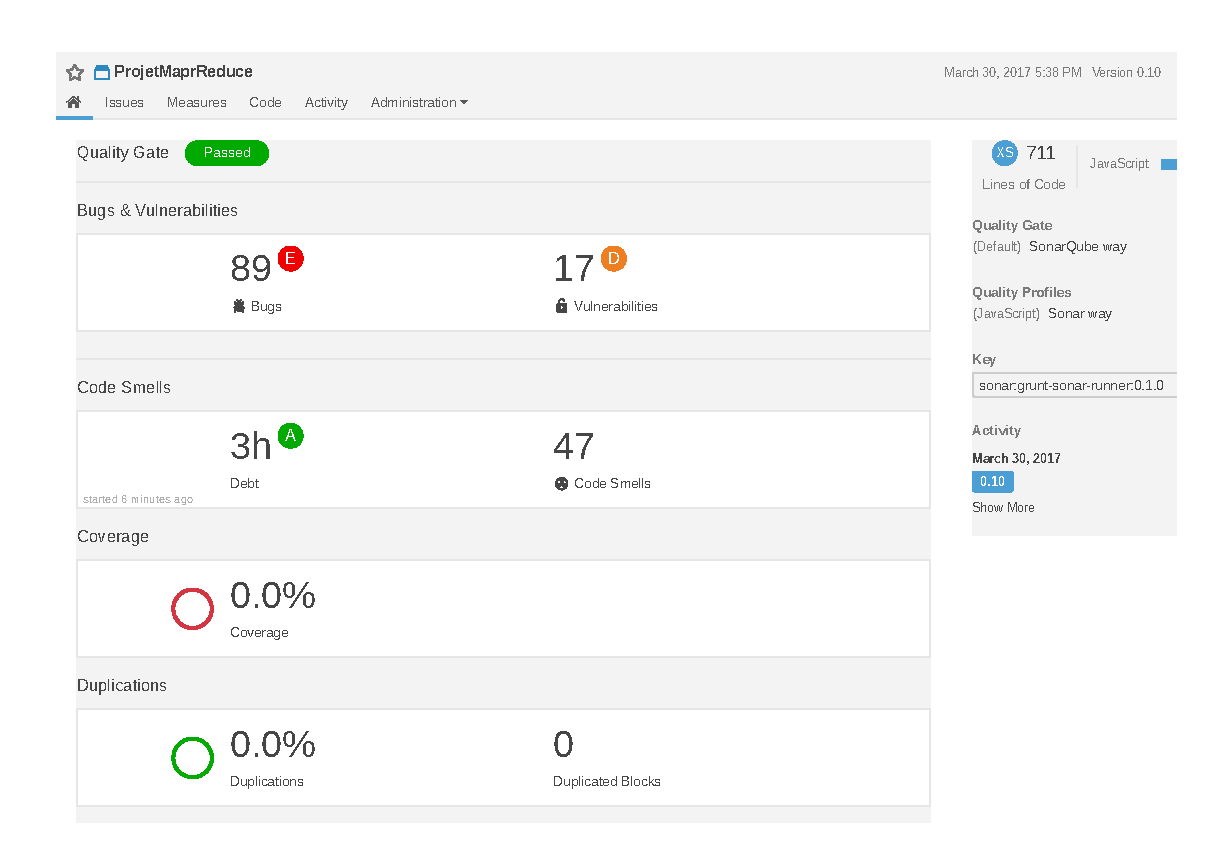
\includegraphics[width=1\textwidth]{images/sonarqube.pdf}
        \caption{Résultats de SonarQube}
	\label{fig:sonarpremierrapport}

\end{figure}

Nous remarquons dans la figure \ref{fig:sonarpremierrapport} la détection de 89 bogues\footnote{Dans SonarQube, les bogues et bogues potentiels sont identifié à partir d'une liste de règles arbitraires.} et 17 vulnérabilités\footnote{Faille de sécurté potentielle. Exemple : Utilisation d'une fonction permettant l'injection de code.}. 

Cependant, {\it SonarQube} considère l'utilisation de la fonction {\tt console.log()} comme une vulnérabilité et rapporte cela comme une erreur sans prendre en compte que cette fonction est principalement utilisée pour les tests unitaires.

Une faille de sécurité nous viens de aussi de l'utilisation de la fonction {\tt eval()} dont nous avons expliqué l'intérêt dans le chapitre \ref{ch:implementation} sur l'implémentation. La fonction {\tt eval()} est nécessaire. Dans le contexte de notre projet, il n'est pas critique de l'utiliser car {\it VisualMapReduce} est réservé à une utilisation locale et privée.

De plus, les résultats sont satisfaisants vis-à-vis de la duplication de code (taux nul) et des heures de dettes techniques\footnote{Les dettes étant le temps qu'une entreprise aurait mis pour déboguer et refactoriser le code.}.
\\
Après avoir revu le code en vue de correction de bogues, les nouveaux résultats obtenus par SonarQube sont ceux de la figure \ref{fig:sonardeuxrapport}.

\begin{figure}[H]
  \centering
    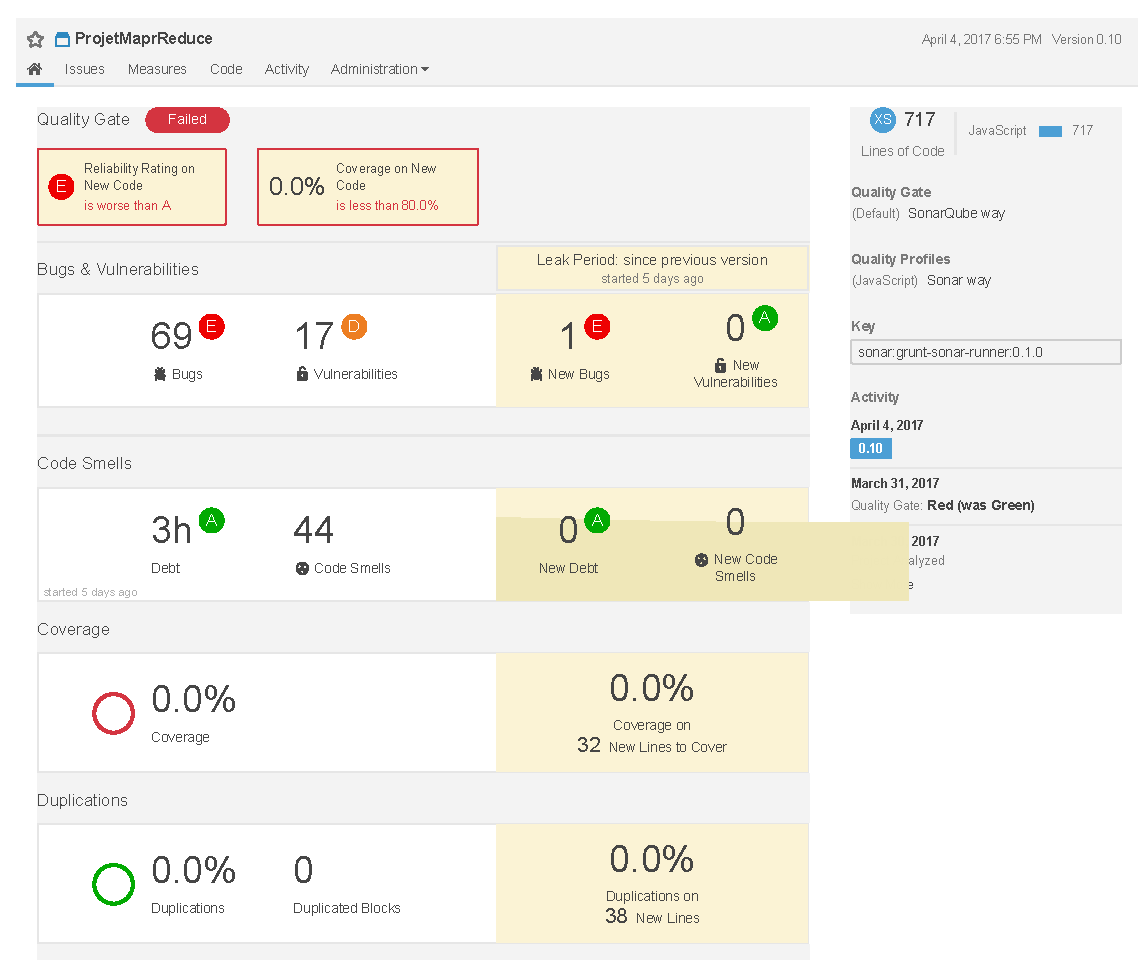
\includegraphics[width=1\textwidth]{images/sonarqube_after_cropped.pdf}
        \caption{Résultats de SonarQube après modification}
        \label{fig:sonardeuxrapport}
\end{figure}
